% Chapter 5

\chapter{Case Study: An R inliner} % Main chapter title

\label{Chapter5} % For referencing the chapter elsewhere, use \ref{Chapter2} 

%----------------------------------------------------------------------------------------

% Define some commands to keep the formatting separated from the content 
\newcommand{\keyword}[1]{\textbf{#1}}
\newcommand{\tabhead}[1]{\textbf{#1}}
\newcommand{\code}[1]{\texttt{#1}}
\newcommand{\file}[1]{\texttt{\bfseries#1}}
\newcommand{\option}[1]{\texttt{\itshape#1}}

%----------------------------------------------------------------------------------------
This Chapter presents experimental results obtained for the RJIT OSR.
The first section describes an implementation of a speculative inliner tool, implemented inside the RJIT compiler, that relies on OSR exits to preserve the program's correctness.
The second section presents benchmarking results obtained while evaluating the OSR inliner, and RJIT OSR main features, i.e., the compensation code to replace invalidated functions, and the \textit{getFreshIR} function.\\

\section{A speculative inliner for RJIT}
\subsection{Justification}\label{section:justificationinlining}
%Dynamic language R 
%function's can be redefined in R, need the OSR typical static opt that is not possible in R
%Used in other papers.
%interesting because implies that we need to clone IR -> put some pressure on our additions.
R is a dynamic language. 
Dynamic programming languages have the particularity to perform, at runtime, common programming behaviors executed during the compilation in static programming languages.
Extending the program, adding code, extending objects and definitions, type setting or modifying the type system are such behaviors that, in dynamic languages, can take place at runtime.
These particularities make certain common static compilation optimizations hard to implement in a dynamic language.
One example of such optimization is inlining (i.e., inline expansion), that replaces a function call site with the callee's body.\\

Chapter \ref{Chapter2} presents the on-stack replacement (OSR) mechanism.
OSR techniques enable to implement \textit{speculative} optimizations, i.e., to transform a function based on the assumption that the result of the transformation will be correct and improve the program's performance at runtime.
If the assumption fails, the OSR mechanisms preserve correctness in the program.
Thanks to this versatile tool, static programming languages optimizations can be performed speculatively in a compiler for a dynamic programming language.\\

In R, and more specifically in RJIT, inlining functions is hard. 
An R function is wrapped in a closure, and might be redefined at any time during the program's execution.
As a result, the only viable way of allowing function inlining in RJIT is to rely on OSR mechanisms.\\

Inlining is an interesting optimization, and its impact on the code performance is hard to predict. 
It holds an important trade-off between time and space, i.e., how much improvement in terms of speed can be obtained, at the cost of some extra space.
Furthermore, excessive inlining might increase register pressure and deplete the instruction cache, therefore decreasing the speed of the program's execution.
Finally, inlining can be viewed as a first step toward other optimizations.
Copying a function's body at its call site enables to enlarge the scope considered by the compiler, and might therefore uncover new optimization opportunities.\\

Apart from being a viable OSR-based speculative optimization in RJIT, inlining allows to put some pressure on the OSR Handler's mechanisms.
First, as explained in chapter \ref{Chapter4New}, the OSR mechanism requires to obtain fresh clones of function bodies via the OSR Handler's functions.
Second, in order to inline a function call, a copy of the callee's body needs to be obtained.
This body, in RJIT OSR, can be obtained through the OSR Handler API.
Function inlining might further force ahead-of-time compilation of the inlined functions, hence enabling us to test every aspect of the functionalities provided by the OSR Handler.\\

RJIT does not gather profiling information that enable to identify good candidates for inlining.
This is, however, far from being a limitation.
On the contrary, it is a perfect case study for OSR mechanisms in R.
Although inlining function calls in R produces unsound compiled code, the OSR mechanism enables to ensure that the program is correct.
As explained in section \ref{justificationgoals}, R performance bottlenecks are consequences of the language semantics.
In the future, on-stack replacement is destined to enable to break R semantics, and to produce unsound, highly optimized code.
Profiling will give insights on whether or not the program might benefit from such optimizations, but is not expected to be able to ensure that any of these transformations is sound.
Not relying on a profiler and blindly inlining function calls, whenever it is possible, illustrates how much flexibility this OSR implementation truly brings to RJIT.\\ 

\subsection{Challenges}
%Function Calls -> how to identify them
%Resolving the function
%Continuation function problem
%IR fresh + AOT behavior
%TODO ENVIRONMENT !!!!!!!!
An OSR-based speculative inliner for RJIT needs to be implemented at the LLVM IR level.
This requires to identify R function calls inside the LLVM IR, extract the callee's SEXP from the environment, and perform the appropriate transformations on the IR.
While relatively simple conceptually, implementing such a mechanism presents several challenges in RJIT.\\

An R function call corresponds to several instructions in the RJIT LLVM IR.
First, a call to the \textit{getFunction} intrinsic is inserted.
The call takes as parameter the AST of the call, stored in the function SEXP constant pool.
This intrinsic enables to resolve, at runtime, the callee. 
To do so it explores the current environment.
If no match is found, it accesses the enclosing environments until either reaching a definition or triggering an error letting the user know that the callee could not be found.
The compiler then emits instructions to load arguments to the function call.
It then inserts a call to the \textit{constant} intrinsic to obtain a pointer to the caller's function pool.
Finally, an ic stub is generated. 
The ic stub takes as arguments the function call arguments, the pointer to the constant pool, the result of the \textit{getFunction} call, the current environment and a pointer to the caller.
When executed once, the ic stub replaces itself with a call to an inlined cached wrapper function dedicated to the callee.
Figure \ref{fig:functioncall} provides a simple R function that performs a function call, and the equivalent LLVM IR generated by RJIT.
Line 5 resolves the callee closure from the environment, line 6 loads the argument to the call, line 7 obtains a pointer to the constant pool, and line 8 performs the call to the ic stub.\\

In the OSR inliner, function calls can be identified by looking for ic stubs.
The OSR inliner has to run on non-instrumented LLVM IR. 
The ic stubs have not yet been replaced by inlined cached wrappers.
Therefore, even though a function call is compiled into several instructions, ic stubs and their arguments are enough to obtain all the information corresponding to a function call.\\

\begin{figure}[h]
\includecode{Code/functionCall.c}
\caption{Example of RJIT LLVM IR for a function call.}
\label{fig:functioncall}
\end{figure}


The OSR inliner needs to obtain a clone of the callee's LLVM IR, in order to inline a function call.
If the callee was never compiled before, the \textit{getFreshIR} function will trigger an AOT compilation of the function.
Since the OSR inliner heavily relies on fresh IR, one challenge is to try to minimize the amount of cloning required in order to perform the transformations.\\

Inlining in R requires to create a dedicated environment for the inlined function.
Implementing a sound name mangler in R is hard. 
It requires to check that fresh names do not collide with parent or child environments.
Furthermore, replacing arguments with their actual values is not semantically correct, due to the way promises are evaluated.
For these reasons, creating a dedicated environment appears to be the only sound solution.\\

The OSR Kit mechanism requires to associate a \textit{toInstrument} clone to every function transformed.
The continuation function has to be a clone of the base function used to generate the optimized one.
One challenge is to carefully implement the inlining in order to limit the number of \textit{toInstrument} functions generated.\\

Finally, all the challenges related to the cloned and continuation functions mentioned in Section \ref{additionalchallenges} need to be considered.
Fixing the LLVM IR requires to go through every instruction in the cloned functions.
As a result, in order to save compilation time, it is important to perform such operations only when they are truly needed.\\

\subsection{Implementation}
%FunctionCall to abstract away the call
%The different mods for inlining.
%The algorithm to inline.

This section describes the implementation of the OSR inliner.
The OSR inliner relies on a special C++ class, called \textit{FunctionCall}, to extract function calls in the LLVM IR and easily access its elements. 
The OSR inliner also provides different modes of execution, that enable more or less aggressive speculative inlining.\\

The FunctionCall class provides a static function, called \textit{getFunctionCalls}, that takes an LLVM IR as input, and extracts the function calls it contains.
For each ic stub call, the function creates an instance of the FunctionCall class. 
A FunctionCall object gives quick access to each element of the function call, i.e., the \textit{getFunction} call instruction, the arguments to the call, and the additional elements of the ic stub call.
The \textit{getFunctionCalls} returns a list of FunctionCall instances.
It is important to note that, for efficiency and better integration, the \textit{getFunctionCalls}, or any similar function that needs to go through the LLVM IR instructions and match a specific pattern, will be able to rely on the pass \& match mechanism being developed in RJIT.
RJIT provides a special matcher mechanism, combined to the LLVM passes implementation, that enables to extract special patterns from the LLVM IR.
One of its main goals is to reduce the number of iterations on the entire LLVM IR, by merging different passes.
Unfortunately, this feature was not yet ready at the time at which the RJIT OSR project was implemented.\\

The OSR inliner implements a very basic, aggressive, speculative inlining algorithm. 
RJIT does not have a profiler or a static analyzer yet.
As a result, the OSR inliner cannot rely on any extra information to decide if a call should be inlined or not.
The OSR inliner proposes different modes of execution, that enable more or less aggressive inlining techniques.
The default mode of execution inlines all the calls inside the current function, as long as a body can be obtained for the callee.
The OSR inliner does not inline recursive calls.
Furthermore, function calls that contain ellipsis or missing arguments are not inlined.
A more agressive mode, called \textit{all inline}, enables to recursively apply the OSR inliner on the body of the functions being inlined.
\\


The OSR inliner implements a very naive inlining algorithm.
All functions calls are extracted from the outer function using the \textit{getFunctionCalls} function.
The OSR inliner then traverses the list of function calls, and groups them by call targets.
The callee's closure can be obtained by looking up the symbol of the function call in the outer function's environment.
In the \textit{all inline} mode, the OSR inliner generates a fully inlined LLVM IR for each different callee, i.e., it inlines all the calls inside each compiled callee. 
In the default mode, the OSR inliner simply calls the getFreshIR method to obtain the callee's LLVM IR.
The OSR inliner creates the toInstrument clone of the outer function.
The toInstrument is used to create the continuation function for each OSR exit inserted in the outer function.
It is wrapped in a valid function SEXP, added to the module, and has a valid IR.
Then, for each different callee, the OSR inliner proceeds as follows: 
\begin{enumerate}
    \item In the body of the callee, update accesses to the constant pool by changing the index to $\text{LENGTH}(\text{CP}_{\text{outer}} + \text{index})$.
    \item Append the callee's constant pool to the outer function's one.
    \item For each function call to the callee:
        \begin{enumerate}
            \item Obtain an unused clone of the callee.
            \item Insert instructions to create a new environment that contains the correct arguments to values mappings, before the ic stub.\label{step:newrho}
            \item Replace all accesses to the environment, i.e., rho argument, in the callee's body by the newly created environment.
            \item Move the callee's body inside the outer function, after the instruction of step \ref{step:newrho}.
            \item Replace all the callee's return instructions by forwarding the return value to a $\phi$-node inserted after the callee's body.\label{step:phinode}
            \item Remove the ic stub.
            \item Replace the ic stub in the transitive mapping between the toInstrument and the outer function by a mapping between the toInstrument corresponding ic stub and the $\phi$-node created in step \ref{step:phinode}.\label{step:updatemap}
            \item Call the insertOSRExit with the outer function as the from function, the toInstrument as the continuation function, instructions that compare the result of the \textit{getFunction} call with the hard coded address of the callee's closure as the OSR condition, and the \textit{constant} call as the transition point, i.e., the instruction that was directly above the ic stub in the original outer function.
        \end{enumerate}
    \item Call the \textit{resetSafePoints} function to correct the optimized function's IR.
    \item Set the optimized function SEXP inside the closure.
    \item Add the optimized function SEXP to the relocations.
    \item Return the closure.
\end{enumerate}

It is important to note that the OSR inliner forces the compilation of every callee. 
As a result, any function contained in the outer function, and inlined, will also be compiled. 
When in the \textit{all inline} mode, they are also fully inlined.
Any subsequent call to a callee will therefore benefit from either a fully compiled, or a fully inlined and compiled version of the function.\\

The continuation function for an OSR exit corresponds to the fully unoptimized base function. 
The toInstrument function is used to generate the continuation function and does not contain any inlined call.
This enables to limit the number of toInstrument functions generated during the transformation of the outer function and avoid triggering OSR exits in cascade.
This also illustrates that, even though it does not correspond to the behavior encouraged by the OSR Kit library, a few careful updates (step \ref{step:updatemap}) to the transitive map enable to preserve a mapping between a base function, and a working copy being modified.
On the other hand, ideally, the continuation function should inline all calls, whenever possible.
This solution can be implemented with on-the-fly compilation of the continuation function, but is not provided in this prototype.\\

The OSR inliner provides a compensation code generator mechanism. 
The compensation code is a simple call to a C++ function, that takes as argument an integer identifier.
The identifier corresponds to a function SEXP containing the toInstrument version.
The C++ function uses the identifier to retrieve the toInstrument function SEXP, and replaces the invalidated function in the closure with this SEXP.\\

Consider the small R functions defined in Figure \ref{fig:simplercode}.
Function $g$ contains two function calls, one to $f$, and another to a function $h$ for which we do not have a definition in the current scope.
The IR displayed in Figure \ref{fig:originalouter} corresponds to $g$.
Lines 3 to 6 correspond to the call to $f$.
Lines 7 to 10 correspond to the call to the unknown function $h$.
Figure \ref{fig:originalinner} provides the LLVM IR of $f$.
We apply the OSR inliner on function $g$.\\

\begin{figure}[h!]
\centering
\includecode{Code/originalR.r}
\caption{A simple R code.}
\label{fig:simplercode}
\end{figure}

\begin{figure}[h!]
\centering
\includecode{Code/originalouter.llvm}
\caption{The original LLVM IR for function g in Figure \ref{fig:simplercode}.}
\label{fig:originalouter}
\end{figure}

\begin{figure}[h!]
\centering
\includecode{Code/originalinner.llvm}
\caption{The LLVM IR for function f in Figure \ref{fig:simplercode}.}
\label{fig:originalinner}
\end{figure}

The result of running the OSR inliner on $g$ is displayed in Figure \ref{fig:inlinedouter}.
The call to $f$ is inlined inside of $g$, between lines 15 and 18. 
Lines 10 to 11 create the dedicated environment for the inlined code.
Lines 5 and 6 correspond to the OSR condition and check that $f$'s address corresponds to the hard coded value seen during the compilation of $g$. 
If this assumption fails, the function jumps to line 28, and triggers the OSR exit by calling the continuation function displayed in Figure \ref{fig:continuationllvm}.
As can be seen between lines 21 and 24, the call to $h$ could not be inlined and was therefore left unmodified.\\

\begin{figure}[h!]
\centering
\includecode{Code/outerInliner.llvm}
\caption{The LLVM IR of g after executing the OSR inliner.}
\label{fig:inlinedouter}
\end{figure}

\begin{figure}[h!]
\centering
\includecode{Code/continuation.llvm}
\caption{The continuation function corresponding to the LLVM IR in Figure \ref{fig:inlinedouter}.}
\label{fig:continuationllvm}
\end{figure}

The continuation function corresponding to the inlined version of $g$ is displayed in Figure \ref{fig:continuationllvm}.
On should note that the continuation function's signature takes as arguments all live values from the from function.
The first three arguments are the same as in the from function.
The last two arguments are respectively the result of the \textit{getFunction} call line 3, and the argument access line 4 in Figure \ref{fig:inlinedouter}. 
Line 3 in the OSR entry block, in Figure \ref{fig:continuationllvm}, is the compensation code used by the OSR inliner.
It enables to replace an invalidated function by its unoptimized version in the corresponding closure. 
As explained previously, it is implemented as a call to a C++ function that takes as argument a unique identifier for the closure.
Lines 7 to 9 are dead code and will be removed in the final compilation steps.\\

\section{Tests}
\subsection{GNUR RJIT vs. Inlining on Shootout benchmarks}

%summary with stats.
%Execution times average per file
%Making it fail did not really changed performances, actually get closer to regular compile if disable.
    %Failure on the benchmarks is hard, because the complete execution flow is hard to manipulate.
        %On microbenchmarks, we were able to make it fail without triggering a recompilation
        %On micro bench, fail with recompilation, i.e., a new function introduced.
    %Consequence of not allowing cascading aborts -> when one failure, we end up with a clean function.
     
%Regular execution, in average 1.03352 ratio, so takes 5% more, max is 1.209086 for spectralnorm-alt.r

%Generating everything and then doing the runs:

This section presents an evaluation of the OSR inliner, based on the Shootout benchmarks~\cite{Shootout}.
As explained in section \ref{section:justificationinlining}, the OSR inliner is a proof of concept, showing that the RJIT OSR enables to break R semantics at a function's level while preserving the overall correctness of the program.
In this section, we compare the all inline mode, i.e., the agressive OSR inliner, against the regular mode, i.e., RJIT without any inlining.
We first report some general numbers and observations gathered in the all inline mode. 
We then compare the execution time obtained in both modes.
Finally, we describe some experiments performed on the OSR Exits.\\

%Stats 
    % No exit. 
        %Kind of good, since we had no profiler. Gives hope that inlining could be much easier, and redefining functions might not be that common. Or simply the benchmark suite is too well written.
        %Describe how we play with it later on.
    % Calls inlined 
        % some bad benchmarks -> list 
            % function contains most of the program
        % Some surprising benchmarks, e.g., pidigits.r 36 calls inlined (out of 237), but resulted in 9747 lines inlined, and reuse of entries over 10 compilations phases.
    % Very little reuse of the IR. Several explanations
        % No recompilation for the moment. Need heuristics based on feedback from the runtime profile. 
        % Probably able to inline user defined functions, since most bench rely on libraries coded in C, and hence no body for them (Builtins). As a result, most calls are inlined during the first JIT compilation. 
        %OSR inliner avoids unnecessary the base version map lookup   

We instrumented the RJIT compiler to gather interesting information about the OSR inliner's execution on the Shootout benchmarks.
A first observation is that none of the benchmarks triggered an OSR exit.
This is a surprising result, since the OSR inliner relied on no profiler, and blindly inlined function calls whenever it could.
We therefore hope that, in most R programs, the redefinition of functions might be rare enough to consider very agressive speculative inlining.
We note, however, that this might be a specificity of the benchmark suite, and recommend to inspect a broader class of R programs before making any assertion.
OSR exits are studied in more details later in this section, and in section \ref{section:osrexitsvsreplacing}.\\

The Shootout benchmarks present very heterogenous results in terms of number of calls inlined.
On all versions of the \textit{revercomplement}, \textit{spectralnorm} and \textit{mandelbrot} benchmarks, only one call was inlined, namely, the benchmark's most important function was inlined in the function serving as entry point for the program.
These benchmarks all contain one function, implementing the benchmark's algorithm.
All calls correspond to built-in functions, which are either library functions implemented in C, or functions with a lot of arguments and default values.
Since the OSR inliner does not support default arguments, these calls could not be considered for inlining.
On the other hand, other benchmarks present more interesting results. 
For example, the \textit{pidigits.r} benchmark's execution led to 36 calls inlined (out of 237 calls, counting calls to built-ins functions), which corresponds to a total of 9747 lines inlined.
In this benchmark, the OSR Handler enabled to provide fresh LLVM IR, without going through the AST to LLVM IR translation, in 10 different compilation modules.
It is also important to note that the JIT compiler is involved less times, in the all inline mode, than in the regular mode.
In fact, the inliner performs AOT compilation of callees, and sets the result inside the corresponding closure.\\

The use of the OSR Handler base version map, for the Shootout benchmarks, yielded a disappointing result.
All the benchmarks, except \textit{pidigit.r}, did not re-use LLVM IR accros different compilation modules.
This, however, has several explanations.
First, the OSR Handler base version map is intended to avoid re-translating ASTs to LLVM IR, for already compiled functions.
A fresh IR is needed when a function is recompiled, or, for the OSR inliner, when a function call is inlined.
RJIT, for the moment, does not collect any profiling information on the program's execution and does not perform any optimization. 
Thus, no recompilation is triggered for unmodified, already compiled, functions.
Another explanation is that the OSR inliner mainly inlines user-defined functions, i.e., the functions defined inside the benchmark (as opposed to built-ins functions).
When the OSR inliner runs on the benchmark's entry point, it recursively inlines calls, hence reaching all the user-defined functions and inlining them whenever it is possible.
Subsequent JIT compilations correspond to calls that the OSR inliner could not inline previously, mainly library functions, that do not call any of the function's cached in the base version map.
As a result, in order to evaluate the efficiency of the base version map, another form of experiment is required.
Section \ref{section:getfreshtest} focuses on the evaluation of the getFreshIR function and the OSR Handler's mechanisms.\\

In a regular execution, the OSR inliner's performance is close to RJIT execution time.
On average, over the entire Shootout benchmarks, in the all inline mode, the execution time is equal to \textbf{1.034} times the regular RJIT execution time.
The slowest execution time registered was for the \textit{spectralnorm-alt.r}, that equals on average 1.21 times the equivalent RJIT execution time.
Figure \ref{fig:execreal5} presents the execution time ratio between the all inline and the regular modes obtained for each benchmark.
We suspect that the overhead introduced by registering fresh IRs, and the OSR inliner's transformations, are the main reasons for this slow down.
In fact, benchmarks that executed faster in the all inline mode than in the regular are the ones cited above, where only one call was inlined.
Moreover, benchmarks that present numerous calls inlined, e.g., \textit{pidigit.r}, have ratios closer to 1.10.
As a result, we suppose that the overhead of blindly inlining function calls is superior to the possible gain in speed. 
We perform a second experiment where the entire compilation overhead is removed.\\

\clearpage
\begin{landscape}
\begin{figure}[h]
    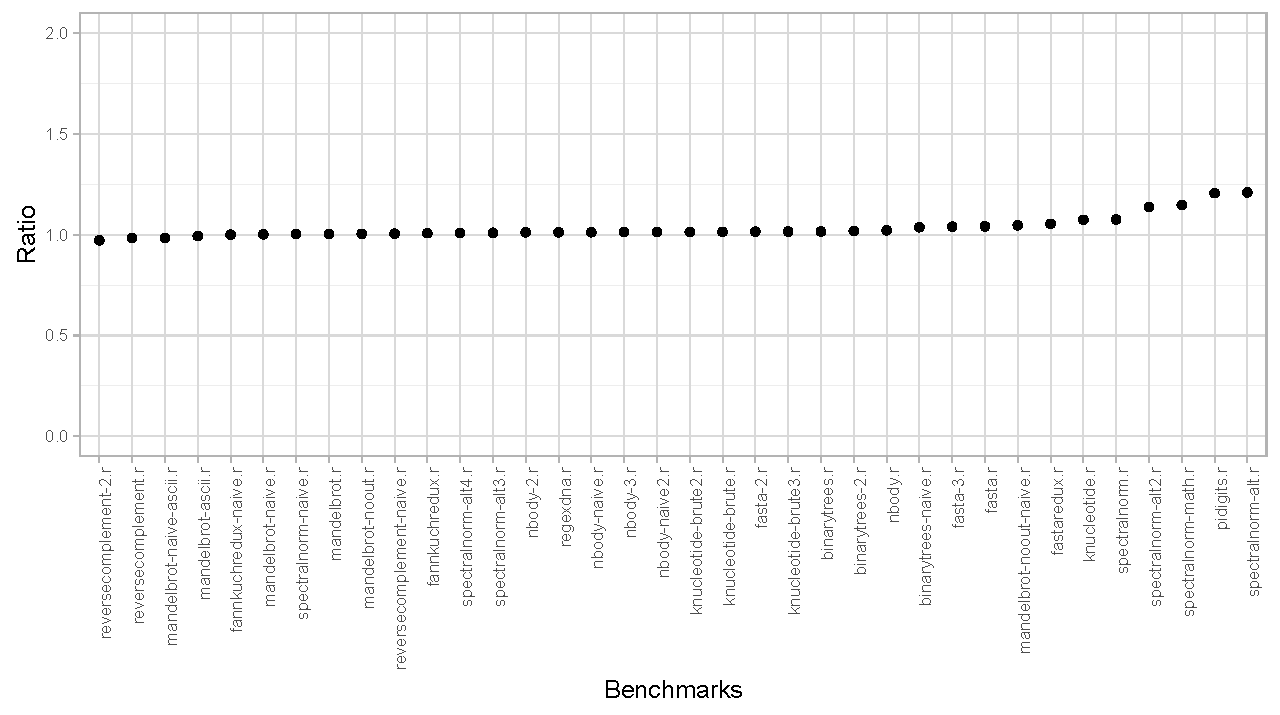
\includegraphics[scale=0.9]{Figures/execReal5}
    \caption{The execution time ratios, per benchmark, between the all inline and the regular mode.}
    \label{fig:execreal5}
\end{figure}
\end{landscape}
\clearpage


Our second experiment measures the average execution time per benchmark, while removing the compilation overhead.
For both modes, we execute the benchmark a first time, so that all functions are compiled. 
We then measure 100 complete executions in the all inline mode, and compare the results to the regular RJIT execution.
Once again, the difference between the two modes of execution is negligible, i.e., the all inline mode's execution is, in average, equal to \textbf{1.004} times the regular RJIT execution.
We notice a small decrease in the average ratio between the two modes of execution.
As before, we look for benchmarks that performed better in the all inline mode than in the regular RJIT one.
Once again, the benchmarks that are made of one long function seem to be faster in the all inline mode.
But, we also notice that other benchmarks, such as \textit{binarytrees-naive.r}, the \textit{fasta}'s, and \textit{nbody}'s, seems to perform better in the all inline mode.
Unfortunately, this is not enough to affirm that the slow down observed in the previous experiment is entirely due to the overhead introduced by the OSR inliner's transformations.
As a result, we conclude that OSR inliner's transformations cannot account for the entire slow down.
Other factors, related to inlining (e.g., register pressure), are also responsible for the slow down.
We measured that the all inline mode leads to more instruction cache misses than the regular execution mode.
However, we failed to find a significative relation between the number of lines inlined in a benchmark, and the increase of icache misses.
For example, a benchmark like \textit{pidigits.r}, in which calls were heavily inlined, displays a smaller icache miss increase than the \textit{knucleotide.r} benchmark.
In order to find a relation between code growth and instruction cache misses, we would need to come up with better statistics about the type of instructions added, and the ones that triggered cache misses.\\

The similarities in terms of execution time, between the two modes, might be explained by the way the OSR inliner inlines calls.
The OSR inliner preserves the function call's logic by creating a dedicated environment for the inlined function.
Creating the environment is one of the dominating costs of a function call.
Implementing a more aggressive inliner, that removes the need to create a dedicated environment for the inlined function, would, potentially, lead to a greater difference, in terms of execution time, compared to the regular RJIT.\\

Forcing OSR exits to be triggered, in the Shootout benchmarks, does not have a significant impact on the performances.
We performed several experiments, where OSR exits were triggered arbitrarily.
Since the OSR inliner introduces a compensation code to replace an invalidated version by a correct one, any OSR exit can be fired only once.
Furthermore, since all OSR Exits exit to a fully non-optimized version of the function, only one OSR exit per function is fired.
As a result, we observed no significant change in the average ratio of execution times in both modes.
We were, however, able to slow down the all inline mode by modifying the OSR inliner such that cascading OSR exits can happen.
On the other hand, these slow downs are meaningless since we purposefully create pathological cases that cannot be generated with the unmodified OSR inliner.\\ 

\begin{table}[h!]
\centering
\resizebox{\textwidth}{!}{%
\begin{tabular}{|l|r|r|r|r|}
\hline
\textbf{Benchmark} & \textbf{\#toInstrument} & \textbf{\#Calls} & \textbf{\#Inlined calls} & \textbf{\#Inlined instructions}\\ \hline \hline
binarytrees-2.r & 2 & 118 & 2 & 166\\ \hline
binarytrees-naive.r & 2 & 115 & 4 & 332\\ \hline
binarytrees.r & 2 & 95 & 2 & 190\\ \hline
fannkuchredux-naive.r  & 1 & 5 & 1 & 26\\ \hline
fannkuchredux.r & 1 & 7 & 1 & 26\\ \hline
fasta-2.r & 2 & 33 & 4 & 556\\ \hline
fasta-3.r & 2 & 40 & 4 & 728\\ \hline
fasta-naive.r & 3 & 34 & 5 & 743\\ \hline
fasta-naive2.r & 3 & 35 & 5 & 819\\ \hline
fasta.r & 2 & 74 & 4 & 428\\ \hline
fastaredux-naive.r & 3 & 41 & 5 & 1055\\ \hline
fastaredux.r & 2 & 40 & 4 & 864\\ \hline
knucleotide-brute.r & 3 & 40 & 3 & 488\\ \hline
knucleotide-brute2.r & 3 & 41 & 3 & 527\\ \hline
knucleotide-brute3.r & 3 & 40 & 3 & 517\\ \hline
knucleotide.r & 3 & 51 & 3 & 490\\ \hline
mandelbrot-ascii.r  & 1 & 17 & 1 & 138\\ \hline
mandelbrot-naive-ascii.r  & 1 & 13 & 1 & 152\\ \hline
mandelbrot-naive.r & 1 & 26 & 1 & 162\\ \hline
mandelbrot-noout-naive.r & 1 & 17 & 1 & 124\\ \hline
mandelbrot-noout.r & 1 & 16 & 1 & 133\\ \hline
mandelbrot.r & 1 & 30 & 1 & 148\\ \hline
nbody-2.r & 2 & 41 & 3 & 264\\ \hline
nbody-3.r & 2 & 42 & 3 & 264\\ \hline
nbody-naive.r & 2 & 49 & 3 & 560\\ \hline
nbody-naive2.r & 2 & 37 & 3 & 370\\ \hline
nbody.r & 2 & 39 & 3 & 274\\ \hline
pidigits.r & 14 & 237 & 36 & 9747\\ \hline
regexdna.r & 1 & 19 & 1 & 95\\ \hline
reversecomplement-2.r & 1 & 17 & 1 & 64\\ \hline
reversecomplement-naive.r  & 1 & 18 & 1 & 74\\ \hline
reversecomplement.r & 1 & 17 & 1 & 58\\ \hline
spectralnorm-alt.r  & 1 & 90 & 1 & 84\\ \hline
spectralnorm-alt2.r & 1 & 90 & 1 & 88\\ \hline
spectralnorm-alt3.r & 1 & 91 & 1 & 118\\ \hline
spectralnorm-alt4.r & 1 & 88 & 1 & 79\\ \hline
spectralnorm-math.r & 1 & 202 & 1 & 35\\ \hline
spectralnorm-naive.r & 1 & 86 & 1 & 76\\ \hline
spectralnorm.r & 1 & 85 & 1 & 72\\ \hline

\end{tabular}}%
\caption{Statistics on OSR inliner's execution on the Shootout benchmarks.}
\label{tab:statsinliner}
\end{table}
\clearpage



\subsection{OSR Exit vs. Replacing the Closure}\label{section:osrexitsvsreplacing}
%OSR Handler enables to replace the continuation
%Avoids triggering the exit all of the time. 
%Need to see if this really improves performances. 
%Should be ...
The OSR Handler enables to add compensation code at the beginning of continuation functions, and replace an invalidated version with a correct one.
This mechanism allows to avoid triggering an OSR exit every time the function is executed.\\

In simple examples, the OSR exit cost can be neglected.
For example, if the OSR condition corresponds to a single, not expensive, comparison, its cost is very small.
On the other hand, if the condition needs to perform an expensive operation, such as a lookup in the environment, or if the OSR exit is located inside a hot loop, executing an invalidated code might increase the program's execution time.\\

We construct a proof-of-concept micro-benchmark to illustrate the gain of performance allowed by the compensation code. 
There are three elements that influence the execution time: 1) The OSR condition, 2) the function call to the continuation function, 3) the execution of ic stubs inside the continuation function.
The call to the continuation function is considered constant.
The two other elements, however, can be made as expensive as we want, very easily.
It is also important to note that for OSR exits contained in loops, without compensation code, these costs appear at each iteration.\\

Figure \ref{fig:microbenchmark} presents the code for our micro-benchmark. 
We insert an OSR exit before each function call, with an OSR condition that retrieves the callee's closure from the environment and always triggers the exit.
The continuation function is such that OSR exits are inserted at each function call, except for the one that triggered the exit.
In other words, every iteration of the loop between lines 4 and 6 will trigger two OSR exits.
The micro-benchmark is small, but contains the interesting features that might impact on the code's performance.
In fact, the continuation function generated for $f_{prime}$ contains two ic stub calls that can never be replaced by faster inlined cached wrappers.
Furthermore, the micro-benchmark is small enough to render the cost of any OSR exit non-negligible compared to the overall execution time.
We execute the benchmark with and without compensation code to replace the invalidated function, and measure the entire execution time.
All measures are performed once all compilations are done, and $g$ has been executed once.
We observe a \textbf{40\%} slow down in the code without compensation compared to the one with compensation.
The micro-benchmark is a fairly simple and common piece of code.
We can therefore be confident that the compensation code has the potential to improve performances in regular R programs.
\\

\begin{figure}[h]
\includecode{Code/microbenchmark.r}
\caption{The micro-benchmark.}
\label{fig:microbenchmark}
\end{figure}


\subsection{OSR Handler getFreshIR vs. Parsing the AST}\label{section:getfreshtest}
%Role of the OSR Handler getFreshIR 
    %Avoid translation step from AST to LLVM IR every time a fresh IR needs to be otbained 
    %Supposed to be faster than walking the AST and generating the llvm ir instructions.
    %Still has some expensive cost, i.e., registering a copy during first compilation, cloning to get a working copy, fixing the IR.
    %Hence need to evaluate its performances.
    %Rely on shootout benchmarks, instrumented such that each function (i.e., 172 functions) is used.

%Overall execution
    %Cost of the registering the working copy 
        %Less than half of the cost of generating  the IR. 
        %Not significant compared to the jitAll cost, i.e., final step to generate the native code.

%Case when the OSR Handler contains a clone for each function.
    %That is the true use case, i.e., functions are jitted, executed. Hot functions are then promoted for optimizations. 
    %Compare time required to parse AST and generate the LLVM IR, and the the time required to get a Fresh and correct IR via the OSR Handler. 
    %Benchmarks are instrumented to have all possible instructions invalidated in the clone, i.e., worst case. 
%Results show that the ratio between getting the working copy and the "translation" is constant, does not vary with the number of instructions in the IR, and is arround 0.33, i.e., it is 3 times faster to get the IR via the OSR Handler than to generate it by reparsing the AST.
%Provide an histogram that represents the frequency of the observed costs for obtaining the IR using both techniques.
%See that with the OSR handler, the costs are concentrated between lalalala. 

The OSR Handler, via the \textit{getFreshIR} and its utility functions, enables to obtain a fresh, non-instrumented, and correct LLVM IR for a function.
This is meant to avoid the translation step from ASTs to LLVM IR every time a fresh non-instrumented IR is needed, e.g., for optimizations.
Obtaining a fresh IR via the OSR Handler, for an already compiled function, is supposed to be faster than walking the entire function's AST and re-generating the corresponding LLVM IR instructions.
The OSR Handler, however, performs some expensive operations, with non-negligible costs, such as registering a copy of the function in the base version map during the function's first compilation, cloning the base version entry to obtain a fresh working copy, and fixing the LLVM IR of clones.
As a result, we evaluate the OSR Handler's mechanisms performance, compared to a regular translation from ASTs to LLVM IR.
To do so, we rely on the Shootout benchmarks~\cite{Shootout}, instrumented such that each function in the benchmarks is used.\\

Registering an entry in the base version map increases the cost of a function's first compilation.
A first experiment therefore consists in comparing the cost of this first compilation via the OSR Handler, and via the regular RJIT mechanism. 
Unsurprisingly, the OSR Handler exhibits poorer performances. 
The reason is that it has to generate the LLVM IR corresponding to the function's AST, as well as cloning the obtained IR and registering the clone in the base version map, while RJIT simply needs to generate the IR.
We evaluate this overhead by breaking down a function's compilation into three steps: 1) the translation, i.e., from GNUR AST to LLVM IR, 2) the registration, i.e, adding an entry in the base version map, 3) the jitAll, i.e., inserting safepoints, patchpoints and generating the native code.
We measure these values over a 1000 compilations of every function implemented in the Shootout Benchmarks.
In average, the cost of registering a function's entry in the base version map is equal to \textbf{0.21} times the cost of the translation, with a standard deviation of 0.07.
If we further compare this result to the overall cost of a complete compilation, i.e., the cost of the translation and jitAll, we obtain a ratio of \textbf{0.004}, with a standard deviation of 0.002. 
From these numbers, we deduce that the cost of registering the entry is negligible compared to the cost of generating the native code.   
As a result, we conclude that the overhead introduced by the OSR Handler to populate the base version map is insignificant compared to the overall execution, and acceptable compared to the translation's cost.\\


The OSR Handler is supposed to improve the RJIT's performances in the presence of optimizations and recompilations.
The expected execution flow is presented in Figure \ref{fig:rjitrecompflow}.
GNUR parses R programs, and constructs the corresponding SEXP containing an abstract syntax tree.
Whenever an element needs to be evaluated, the RJIT compiler is invoked. 
The SEXP is translated into LLVM IR, instrumented, compiled to native code, and wrapped into a native SEXP before being returned to GNUR.
When a function becomes hot, i.e., when it has been executed several times, it becomes a candidate for recompilation and optimizations.
This corresponds to the real use case of the OSR Handler's mechanisms.
The OSR handler enables to skip the re-parsing of the AST and corresponds to the "\textit{recompilation}" arrow in Figure \ref{fig:rjitrecompflow}.
As a result, we need to evaluate the cost of obtaining a non-instrumented and correct IR from the OSR Handler, when the base version map already contains an entry for the function, and compare it to the cost of generating the IR from the AST.
We therefore perform a second experiment, where the OSR Handler has a fully generated base version map.
In this experiment, we further ensure that every call instruction inside the clones obtained via the \textit{getFreshIR} function need to be fixed.
This corresponds to the worst case scenario for the execution of the \textit{resetSafepoints} function, and thus provides an upper bound on the performance evaluation.\\

\begin{figure}[h!]
\center
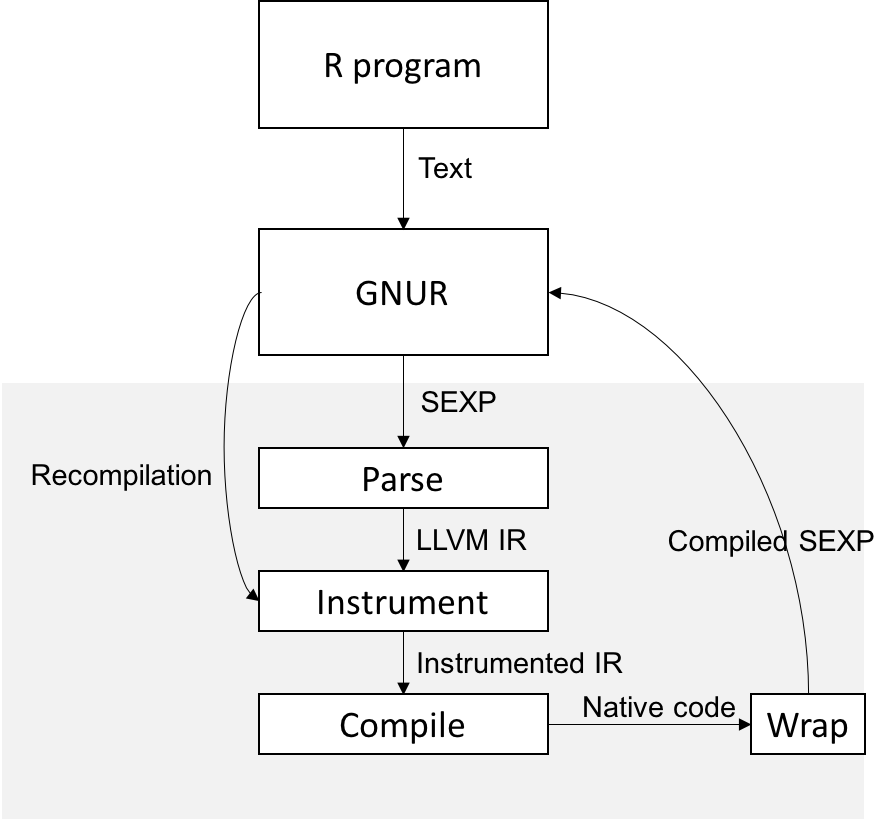
\includegraphics[scale=0.5]{Figures/RjitFlowRecomp}
\caption{The RJIT detailed compilation and recompilation flow.}
\label{fig:rjitrecompflow}
\end{figure}

Our second experiment yields encouraging results.
A first observation is that the time ratio between obtaining the IR via the OSR Handler and via RJIT translation is constant, regardless of the number of LLVM IR instructions generated, with a median value at \textbf{0.33}. 
In other words, it seems that obtaining a fresh and correct IR, for an arbitrarily sized function, via the OSR Handler, is in average at least \textbf{three} times faster than generating it from the AST.
These results can further be improved if less instructions need to be fixed.
As explained in Section \ref{section:cleanerIR}, a future solution would be to save an entire module per function in order to avoid having to fix LLVM IR instructions.
With this solution, the cost of obtaining a fresh non-instrumented IR would include the cost of loading an LLVM module into the current compilation module. 
Since it is not part of our implementation, we do not provide any estimation for this cost.\\

\begin{figure}[h]
    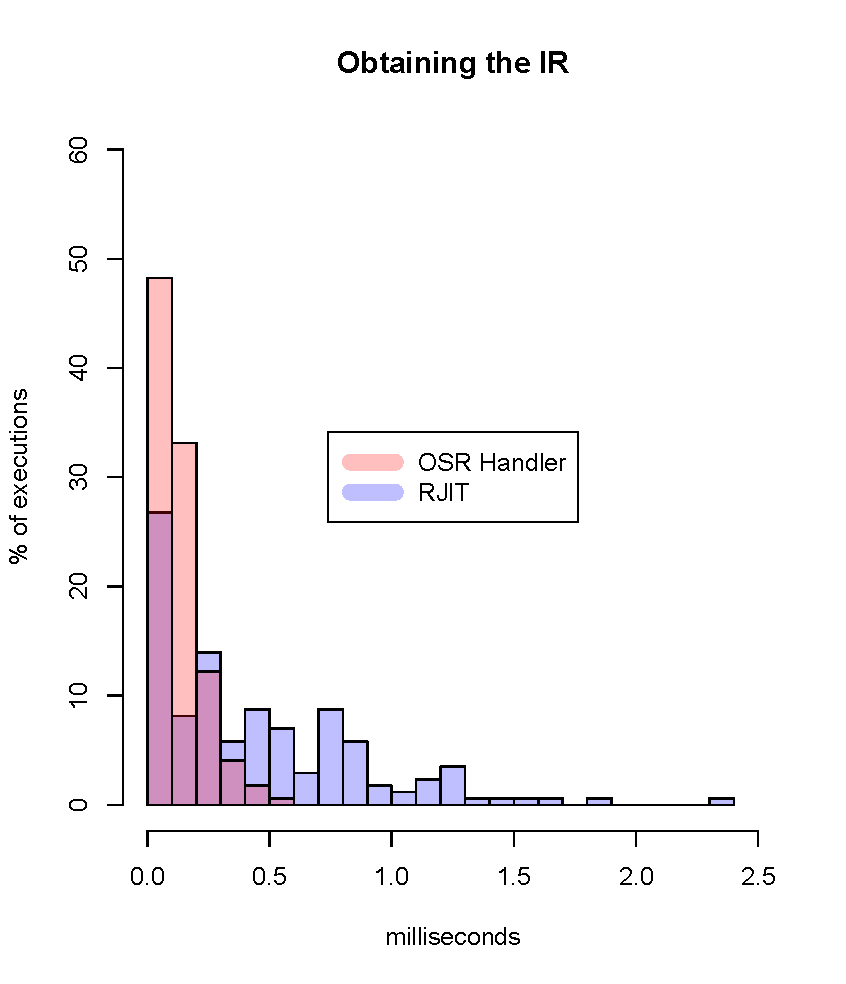
\includegraphics[scale=0.9]{Figures/withoutJitAll2}
    \caption{OSR Handler versus RJIT: histogram of the time required to obtain a non-instrumented and correct IR for all the functions in the Shootout benchmark.}
    \label{fig:withoutJitAll}
\end{figure}

Figure \ref{fig:withoutJitAll} presents an histogram corresponding to our second experiment.
The histogram represents the distribution of times observed to obtain a fresh, non-instrumented, and correct IR, via RJIT and via the OSR Handler, on the same set of functions.
For the OSR Handler, all executions took less than 0.6 milliseconds, which represents one quarter of RJIT's time span.
In RJIT, 30\% of executions are still above 0.6 milliseconds.
For the OSR Handler, 81.4\% of the executions are under 0.2 milliseconds.
For RJIT, only 34.9\% took under 0.2 milliseconds.\\

In the light of these results, we conclude that avoiding to generate fresh IRs from ASTs for already compiled function yields better results, i.e., three times faster, regardless of the number of instructions contained in the function, and even when all call instructions are invalidated.
We can further affirm that the getFreshIR performance compensates the overhead introduced while registering an entry in the base version map.\\

The OSR handler introduces a memory overhead that can be quantified.
For each live and compiled function, the OSR Handler contains a function SEXP that points to the same constant pool, and contains a clone of the function's non-instrumented LLVM IR.
Since, for the moment, a garbage collection induces a flush of the OSR Handler's base version map, i.e., all entries are deleted, we can say that only live functions, compiled since the last garbage collection, have an entry in the OSR Handler.
Flushing the entire base version map is too drastic. 
A more subtle implementation would flush only entries corresponding to collected closures.
This requires, however, a more complex interaction with the garbage collector, that we did not have time to implement.
Finally, the solution described in section \ref{section:cleanerIR} will exhibit similar space costs, but will also be easier to integrate with the garbage collector.\\
